\documentclass{report}
\usepackage[extreme]{savetrees}
\usepackage{wrapfig}
\usepackage{graphicx}
\graphicspath{{./images/}}
\usepackage{amsthm}
\usepackage{siunitx}
\usepackage{url}
\usepackage{subfig}
\usepackage{lscape}
\usepackage{amsmath}
\usepackage{tikz}
\usepackage{mathdots}
\usepackage{yhmath}
\usepackage{cancel}
\usepackage{color}
\usepackage{siunitx}
\usepackage{array}
\usepackage{multirow}
\usepackage{amssymb}
\usepackage{gensymb}
\usepackage{tabularx}
\usepackage{booktabs}
\usetikzlibrary{fadings}
\title{Marketing Training Report}
\author{Tuneer Bhattacherjee\\Employee Id: 514370\\BhattacherjeeT@indianoil.in}
\makeindex
\begin{document}
	\maketitle
	\pagebreak
	\tableofcontents
	\pagebreak
	\chapter{Sanand Bottling Plant - Day 1 (13.08.2019)}
	\section{Important Terms and Abbreviations}
	\begin{itemize}
		\item OISD = Oil Industry and Safety Directorate
		\item TT= Tanker Trucks
		\item Cavitation = Cavitation is a phenomenon in which rapid changes of pressure in a liquid lead to the formation of small vapor-filled cavities, in places where the pressure is relatively low.When subjected to higher pressure, these cavities, called "bubbles" or "voids", collapse and can generate an intense shock wave. These shock waves can damage pumps/motors.
		\item CFM= Cubic Feet per Minute
		\item SO= State Office
		\item HO= Head Office
		\item DOA= Delegation of Authority
		\item BCW= Blue Collar Workers
	\end{itemize}
	\section{Introduction to Sanand LPG Bottling Plant - Salient Points}
	\textit{Faculty: Shri. Joydev Ojha, DGM(P), Sanand BP}
	\begin{figure*}
		\centering
		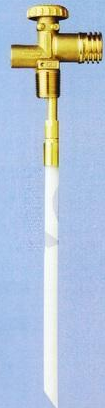
\includegraphics{lot_valve}
		\caption{LOT Valve}
		\label{lot_valve}
	\end{figure*}
	\begin{figure*}
		\centering
		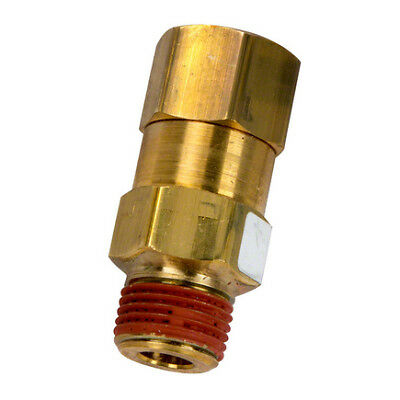
\includegraphics{sc_valve}
		\caption{SC Valve}
		\label{sc_valve}
	\end{figure*}
	\begin{itemize}
		\item Due to low land prices and government push, this particular bottling plant has much more space than what is required under the OISD guidelines.
		\item In addition to that, there is a 66 acre buffer area which is not required anymore according to the latest OISD guidelines so, the plant "occupier" or location in charge Shri. Joydev Ojha, DGM(P) has decided to utilize it to benefit the corporation in the following ways:-
		\begin{itemize}
			\item A 8MW solar plant was established in the buffer area which generates about Rs.3 lacs of electricity per day, part of which is used up by the factory and part is distributed to other IOCL facilities via the grid. It is important to note that according to the some regulations in the Gujrat solar power consumption policy, IOCL at max can only generate 50\% of their net electricity demand if they wish to stay on grid and share their power with other IOCL facilities using the same. This facility covers 66 acre of the buffer area. 
			
			\item  A 2 acre lube storage facility (CFA). It is important to note here that lube being a high flashpoint product is an ``excluded product''. Therefore, storing it in buffer areas donot raise any safety concerns.
			
			\item 4 acres are being delegated to the pipelines division to facilitate the Kandla-Gorakhpur pipeline.
			
			
		\end{itemize}
		\item Product is sourced into the bottling plant using approximately 100 LPG TTs of 18-20 MTs from the following sources -
		\begin{itemize}
			\item Kandla port
			\item Pipawa port
			\item Varoda refinery
			\item Reliance refinery, Jamanagar
			\item Essar refinery, Jamnagar etc.
		\end{itemize}
	
		\item There are 8 TLDs which takes about 3-4 hours to completely decant all the trucks and this happens in about 4 batches a day.
		
		\item Storage of LPG is done as follows:-
		\begin{itemize}
			\item 3 Horton Spheres 1400 MT,1200 X 2 MT
			\item 1 Stationary Vessel ie. Bullet 150 X 4 MT
		\end{itemize}
		Therefore, net storage capacity = $1400+12 X 1200+150X4 = 4400 MT$
		\item Decantation is done via pressure difference using a vapour compressor in the following steps:-
		\begin{itemize}
			\item First vapour of TT is pressurized by taking vapour from vessel. This forces liquid LPG to move from TT to vessel.
			\item Then, liquid valve is closed and then vapour is sucked from the tanker using vapour suction.
		\end{itemize}
		This method is preferred over simply using pumps to pump the LPG from TT to vessel because if the pump pulls vapor by mistake, that will lead to cavitation.
		\item There are 3 carousels - 1400 cylinders/hour X 2 and 1600 cylinders per hour.
		\item The 3 carousels are fed by 3 pumps - 110 , 90, 36 X 2 CFM each with a max capacity of 6000 cylinders per month therefore, the net capacity would be approximately 18000 per month, but generally only about 15000 are required to be produced as per guidance from SO.
		\item The following requirement from SO side is generated by a computer model which takes the following factors into account -
		\begin{itemize}
			\item Bulk receiving cost
			\item Capacity of plant
			\item Demand from market
			\item Transportation cost from plant to market
		\end{itemize}
		\item There are 2 types of valves in cylinders ie. Self Closing Valve (SC) \ref{sc_valve}and Liquid Off Take Valves (LOT) \ref{lot_valve}.
		\item Delivery within 24 hours to distributor.
		\item There are baffle plates in LPG TTs to arrest momentum of the fluid thereby causing less hindrance to the driver.
	\end{itemize}
	\section{Roles and Responsibilities - Salient Points}
	\textit{Faculty: Shri. Joydev Ojha, DGM(P), Sanand BP}
	\begin{itemize}
		\item Occupier has he role responsibility and has the power of attorney
		\item The occupier then delegates the responsibility /authority to other officers below him via DOA guidelines.
		\item Finally the grass root users of official authority are Grade 'A' Officers who get the work done by the BCW in company payroll and contractors.
	\end{itemize}
	\section{LPG Plant Layout - Salient Points}
	\textit{Faculty: Shri. B.H. Bharti, SM(P), Sanand BP}
	\begin{itemize}
		\item There are four sizes of BPs based on net production per annum-
		\begin{enumerate}
			\item less than 6000 ---- Micro
			\item between 6000 to 22000 ---- Mini
			\item between 22000 to 68000 ---- Major
			\item greater than 68000 ---- Mega
		\end{enumerate}
		Based on information given above the average production per month of Sanand BP is 15000 therefore appx. production per annum 15000 X 12 = 180000 which is greater than 68000. Therefore, Sanand BP is a Mega Plant.FacuFaculty: Shri. Joydev Ojha, DGM(P), Sanand BPlty: Shri. Joydev Ojha, DGM(P), Sanand BP
		\item Vapour seals are used in water drains so that LPG vapour (which is heavier than air) cannot travel outside the plant licensed area where it can catch spark and ignite thereby causing grave fatalities and carry the ignition to plant and cause an even bigger calamity.
		\item Types of storage at any LPG facility can be as follows:-
		\begin{itemize}
			\item Above ground storage- Bullets, Horton Spheres, Mounded Storage
			\item Under ground storage
			\item Cavern storage
			\item Refrigerated storage tank @ \ang{-42}C and atm pressure
		\end{itemize}
		\item Minimum of 3 vessels are to be kept at a plant.
		\item Storage vessel should be filled upto 84-85\% to keep room for LPG expansion with change of temperature, failing this, risk of explosions due to expansions are considerably increased which renders such operating procedure ineffective and useless. 
		\item Mimimum compressor air pressure for carousel is 5.5 kg/cc and for the latest fully automatic carousel it is 6 kg/cc
		
		
	\end{itemize}
	\section{FAQs}
	\begin{description}
		\item[What is the standard pressure in a LPG T/T?] answer
		\item[What is the minimum pressure in a LPG cylinder?] 15 kg/cc
		\item[What factors go into the calculation of production requirement of a bottling plant?] answer
		\item[Why are LOT cylinders required?] Because Liquid Off Take (LOT) Cylinders have valves with pipes which go down to the lower part of the cylinder therefore, allowing it to draw liquid from the cylinder which may then be used to evaporate at a higher rate along with other LOT cylinders, thereby creating enough vapour for large burners, furnaces etc. Therefore, it is generally used for commercial/industrial purposes.
	\end{description}
\end{document}